\documentclass{article}

% Language setting
% Replace `english' with e.g. `spanish' to change the document language
\usepackage[portuguese]{babel}

% Set page size and margins
% Replace `letterpaper' with `a4paper' for UK/EU standard size
\usepackage[a4paper,top=2cm,bottom=2cm,left=3cm,right=3cm,marginparwidth=1.75cm]{geometry}

% Useful packages
\usepackage{amsmath}
\usepackage{subcaption}
\usepackage{graphicx}
\usepackage[colorlinks=true, allcolors=blue]{hyperref}

\title{Trabalho Prático 01}
\author{Luciano Stork}

\begin{document}
\maketitle

\begin{abstract}

O avanço tecnológico tem impulsionado a produção e o compartilhamento de imagens digitais em uma escala sem precedentes. No entanto, o aumento exponencial no volume de dados gerados cria desafios significativos em termos de armazenamento, transmissão e processamento eficientes dessas imagens. Nesse cenário, técnicas de compressão de dados desempenham um papel crucial na mitigação desses desafios, permitindo a redução do tamanho dos arquivos sem comprometer significativamente a qualidade visual.

Uma dessas técnicas é o Run-Length Encoding (RLE), um método de compressão simples e eficaz que se destaca por sua capacidade de reduzir a redundância em conjuntos de dados sequenciais. O RLE é particularmente adequado para dados que exibem certas características, como uma imagem com conjunto restrito de cores e grandes áreas de cor homogênea. Nessas situações, o RLE pode alcançar taxas de compressão significativas, reduzindo o tamanho do arquivo de imagem de forma substancial.

Este trabalho tem como objetivo explorar a aplicação do RLE em imagens coloridas que apresentam essas características específicas, com o intuito de otimizar a compressão e reduzir o consumo de recursos de armazenamento e largura de banda. Ao adaptar e aprimorar o RLE para lidar com imagens coloridas, pretende-se explorar suas capacidades em capturar a redundância presente nessas imagens e realizar uma compressão mais eficiente.

Além disso, propõe-se a criação ou aprimoramento de um formato de texto específico para armazenar os dados da imagem após a compressão com RLE. Esse formato incluirá um cabeçalho que permite arquivar metadados e parâmetros relevantes da compressão, incluindo informações da própria imagem, facilitando sua reconstrução e interpretação posterior.

Dessa forma, este projeto busca não apenas aprimorar a técnica de compressão de dados utilizando o RLE, mas também propor uma abordagem abrangente para o armazenamento e compartilhamento eficientes de imagens com características específicas, contribuindo para a otimização dos recursos de armazenamento e transmissão em ambientes onde tais imagens são amplamente utilizadas.

\end{abstract}

\section{Implementação do RLE para Imagens com Cores Limitadas:}
\subsection{Desenvolvimento de um algoritmo RLE adaptado para imagens que utilizam um conjunto restrito de cores:}

Inicialmente, conforme sugerido pelo professor em sala de aula, pensei em abordar a compressão da imagem a partir da função \textbf{rleenco} e \textbf{rledeco}, disponíveis no pacote \textbf{communications} do Matlab. No entanto, a versão que possuo instalada não foi capaz de reconhecer tal biblioteca; sendo necessário, portanto, desenvolver funções similares ao funcionamento desses encapsulamentos citados. Desse modo, foram desenvolvidas as funções \textit{custom\_rle\_encode} e \textit{custom\_rle\_decode}

\begin{itemize}
    \item Na função \textit{custom\_rle\_encode}, é realizada a codificação Run-Length Encoding (RLE) em um vetor de entrada chamado \textit{message}. Inicialmente, uma matriz vazia chamada \textit{encoded\_data} é criada para armazenar os dados codificados resultantes da compressão RLE. Além disso, a variável \textit{count} é inicializada com o valor 1. Esta variável será usada para contar as repetições de cada valor no vetor \textit{message}.
    Em seguida, um loop é iniciado para percorrer cada elemento do vetor \textit{message}. Dentro do loop, verificamos se o elemento atual é igual ao próximo elemento e também se não estamos no último elemento do vetor analisado. Se ambas as condições forem verdadeiras, significa que encontramos uma sequência de valores \textbf{repetidos}. Nesse caso, incrementamos o contador \textit{count} para acompanhar o número de repetições.
    Quando encontramos um elemento que não é igual ao próximo, significa que a sequência de valores repetidos terminou. Então, adicionamos o par \textbf{(contagem, valor)} à matriz \textit{encoded\_data}, onde a contagem representa o número de repetições e o valor é o próprio elemento. Por fim, o contador \textit{count} é reiniciado para 1 para o próximo valor a ser processado no vetor \textit{message}. Após o loop, a função retorna os dados codificados armazenados na matriz \textit{encoded\_data}.

    \item Já a função \textit{custom\_rle\_decode} é responsável por decodificar os dados codificados anteriormente. Inicialmente, uma matriz vazia chamada \textit{decoded\_data} é criada para armazenar os dados decodificados resultantes da compressão RLE.
    Em seguida, um loop é iniciado para percorrer a mensagem codificada. A cada iteração do loop, dois elementos consecutivos da matriz \textit{encoded\_data} são extraídos. O primeiro elemento representa o \textbf{número de repetições} \textit{(count)} e o segundo elemento representa o \textbf{valor que foi repetido} \textit{(value)}.
    Para decodificar os dados, o valor \textit{value} é replicado \textit{count} vezes e adicionado à matriz \textit{decoded\_data}. Isso é feito utilizando a função \textit{repmat}, que replica o valor \textit{value count} vezes.
    Após percorrer toda a mensagem codificada, a função retorna os dados decodificados armazenados na matriz \textit{decoded\_data}.
\end{itemize}

Por questões de complexidade do código em razão do impasse de não reconhecimento do Matlab às funções nativas, optei por fazer todo o processamento em imagem com tons de cinza. Isso por conta do custo de processamento da minha máquina a imagens coloridas e pelo consequente tempo de resposta do programa, que alcançava valores onerosos pensando em disponibilidade para com o desenvolvimento proposto.
Entretanto, para o caso de imagens coloridas, basta extrapolar a ideia para as três dimensões (RGB), trabalhando ou com três vetores, ou com uma matriz.

\subsection{Incorporação de estratégias específicas para otimizar a compressão em áreas homogêneas de cor:}

Ao analisarmos os códigos fornecidos das funções \textit{custom\_rle\_encode} e \textit{custom\_rle\_decode}, podemos identificar oportunidades para aprimorar a compressão em áreas homogêneas de cor em imagens. Uma abordagem inicial seria a identificação dessas áreas antes da aplicação do algoritmo RLE. Isso pode ser realizado por meio de uma análise dos valores de \textbf{cor dos pixels adjacentes}, procurando por regiões com variações mínimas nos valores de cor. Uma vez identificadas essas áreas, podemos aplicar estratégias específicas de compressão para otimizar o processo.

Uma técnica comum é a codificação diferencial, onde em áreas homogêneas armazenamos apenas as diferenças entre os valores de cor consecutivos, em vez de armazenar cada valor individualmente. Essa abordagem pode reduzir significativamente a quantidade de dados a serem armazenados, especialmente em áreas onde os valores de cor são constantes ou mudam de forma gradual.

Além disso, podemos considerar a segmentação adaptativa da imagem, dividindo-a em regiões com características similares e aplicando diferentes técnicas de compressão em cada região. Por exemplo, podemos aplicar o RLE em áreas homogêneas, enquanto em áreas mais complexas ou com padrões irregulares, podemos utilizar outros algoritmos de compressão mais eficazes.

Podemos, ainda, considerar a inclusão de metadados no arquivo comprimido, que descrevem as áreas homogêneas detectadas, incluindo suas posições e tamanhos. Esses metadados podem ser úteis durante o processo de descompressão para identificar e decodificar eficientemente as áreas homogêneas, contribuindo para uma recuperação precisa da imagem original.

Ao incorporar essas estratégias específicas de compressão, podemos otimizar significativamente o processo de compressão de imagens, especialmente em áreas homogêneas de cor, resultando em taxas de compressão mais eficientes e arquivos comprimidos menores. Saliento que por questões de complexidade, este trabalho pautou-se apenas na descrição das possíveis melhorias do código principal para atender com melhor desempenho a atividade proposta.

\section{Avaliação do Impacto da Homogeneidade de Cor:}
\subsection{Análise do impacto da homogeneidade de cor na eficiência do RLE:}

A homogeneidade de cor em uma imagem refere-se à presença de grandes áreas com cores similares ou idênticas. Essas áreas são caracterizadas pela repetição de pixels com valores de cor próximos ou idênticos, o que pode resultar em redundância de dados. O Run-Length Encoding (RLE) é uma técnica de compressão de dados que se beneficia diretamente desse tipo de redundância, pois compacta sequências repetidas de valores em uma representação mais compacta.

No entanto, o impacto da homogeneidade de cor na eficiência do RLE pode variar dependendo de vários fatores, incluindo a distribuição e o tamanho das áreas homogêneas na imagem. É interessante analisar mais detalhadamente como a homogeneidade de cor pode influenciar a eficiência do RLE:

\begin{itemize}
    \item Redundância de Dados: Em áreas onde a cor é altamente homogênea, ou seja, onde há repetição significativa de valores de cor, o RLE pode comprimir esses dados de forma muito eficiente. Isso ocorre porque o RLE identifica sequências repetidas e as substitui por uma representação mais compacta que inclui o valor da cor e o número de repetições.

    \item Tamanho das Áreas Homogêneas: O tamanho das áreas homogêneas é um fator crucial. Quanto maior a área homogênea, maior será o potencial de compressão do RLE, pois uma sequência repetida de pixels será mais longa. Grandes áreas homogêneas podem resultar em uma redução significativa do tamanho do arquivo após a compressão com RLE.

    \item Distribuição das Áreas Homogêneas: A distribuição das áreas homogêneas na imagem também é importante. Se as áreas homogêneas estiverem dispersas por toda a imagem, o RLE poderá encontrar mais oportunidades para compressão, pois diferentes partes da imagem apresentarão repetição de cores. Por outro lado, se as áreas homogêneas estiverem concentradas em uma região específica, o impacto na compressão pode ser menor.

    \item Variação da Cor: Em imagens com variações sutis de cor, o RLE pode não ser tão eficiente, especialmente se as áreas homogêneas forem pequenas ou se houver transições suaves entre as cores. Nesses casos, a repetição de valores de cor pode não ser tão evidente, resultando em uma compressão menos eficaz.
\end{itemize}

Desse modo, percebe-se que a homogeneidade de cor tem um impacto significativo na eficiência do RLE. Em geral, áreas homogêneas de grande extensão tendem a ser comprimidas de forma muito eficaz pelo RLE, enquanto variações sutis de cor podem resultar em uma compressão menos eficiente. Ao considerar o uso do RLE para compressão de imagens, é essencial analisar a distribuição e o tamanho das áreas homogêneas para determinar o potencial de compressão e avaliar o impacto esperado na eficiência da compressão.

\begin{figure}[htbp]
    \centering
    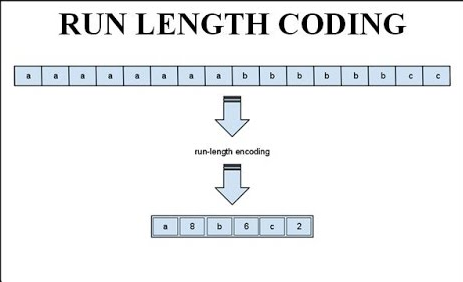
\includegraphics[width=0.5\textwidth]{RLE.png}
    \caption{Lógica de funcionamento do RLE.}
    \label{fig:imagem}
\end{figure}

\subsection{Exploração de técnicas específicas para identificação e tratamento de grandes regiões com cores uniformes:}

A identificação e o tratamento de grandes regiões com cores uniformes em imagens suprem, nesse cenário, um papel fundamental em diversas aplicações de processamento de imagem, como segmentação, compressão e análise de conteúdo visual. Essas regiões, caracterizadas pela consistência e homogeneidade das cores, frequentemente contêm informações importantes e representam elementos distintos na imagem. Neste contexto, a exploração de técnicas específicas para identificação e tratamento dessas regiões é essencial para aprimorar a eficiência e a qualidade das análises realizadas sobre as imagens.

Uma das abordagens mais comuns para identificar grandes regiões com cores uniformes é a segmentação por limiarização. Essa técnica envolve a definição de um limite de intensidade de cor, onde pixels com valores acima desse limite são atribuídos a uma categoria e pixels abaixo do limite a outra. A limiarização é uma técnica simples e eficaz, adequada para imagens com regiões de cores bem definidas e contrastantes.

Além disso, técnicas de agrupamento baseadas em cores, como o algoritmo K-means, oferecem uma abordagem poderosa para identificar regiões com cores uniformes. Esses algoritmos agrupam pixels semelhantes em termos de cor em clusters, permitindo a identificação de regiões com características cromáticas semelhantes. O K-means é especialmente útil quando se trata de identificar regiões com cores que não são facilmente separáveis por um único limite de intensidade.

Outra estratégia importante é a aplicação de filtros de suavização ou filtragem de ruído. Esses filtros têm o objetivo de reduzir a variabilidade de cor nos pixels da imagem, suavizando transições abruptas e realçando regiões com cores uniformes. Técnicas como a média, mediana e filtro de Gauss são comumente utilizadas para esse fim, proporcionando uma abordagem robusta para identificar e tratar grandes regiões com cores uniformes.

Em conjunto, essas técnicas oferecem um conjunto abrangente de ferramentas para a identificação e tratamento de grandes regiões com cores uniformes em imagens. Ao explorar essas técnicas, é possível aprimorar a segmentação, compressão e análise de conteúdo visual, permitindo uma compreensão mais profunda e precisa das informações contidas nas imagens.

\section{Proposta de Formato de Arquivo para Dados Comprimidos:}
\subsection{Desenvolvimento ou proposta de um formato de arquivo binário ou texto para armazenar os dados da imagem após a compressão RLE:}

Obviamente, a tarefa de salvar os metadados obtidos durante o processo de compressão em um arquivo de texto também é um ponto importante que demanda análise das estratégias corretas para maior assertividade. Para isso, inicializamos no código uma estrutura de blocos de metadados, na qual armazenamos informações relevantes sobre a compressão RLE aplicada à imagem. Esses metadados incluem o formato de compressão utilizado, a largura e altura da imagem original, o tamanho do arquivo comprimido e a taxa de compressão obtida.

Para armazenar esses metadados no arquivo de texto \textit{metadados.txt}, primeiro convertemos os dados comprimidos em uma sequência de caracteres utilizando a função \textit{sprintf}. Em seguida, escrevemos os metadados e os dados comprimidos no arquivo de texto. Utilizamos um loop para percorrer os campos da estrutura de metadados e escrevemos cada campo e seu valor correspondente no arquivo. Após escrever os metadados, escrevemos também os dados comprimidos, precedidos pela indicação \textbf{"Dados\_Comprimidos:"}, no arquivo de texto. Por fim, fechamos o arquivo após concluir a escrita.
Cito que a escolha por um formato de arquivo \textit{.txt} pautou-se na facilidade de visualização do conteúdo do mesmo, tanto para entender o que estava sendo feito no processo de compressão, quanto para conferir se o produto dos códigos condizia com a lógica do RLE. Essa abordagem permite armazenar de forma organizada e legível os metadados da compressão e os dados comprimidos em um arquivo de texto, facilitando o compartilhamento e a reestruturação das informações relacionadas à compressão da imagem.

\subsection{Utilização de cabeçalho para arquivar metadados e parâmetros relevantes da compressão ou da imagem:}

Os metadados são informações descritivas que fornecem contexto e detalhes sobre os dados contidos em um arquivo. Eles descrevem as características dos dados, como seu formato, origem, conteúdo e outras propriedades relevantes; ajudando a contextualizar e interpretar os dados armazenados, fornecendo informações adicionais, que muitas vezes se camuflam dentre as diversas informações disponibilizadas, além dos próprios dados.

No exemplo tratado pelo algorimo em questão, o arquivo de texto contém metadados relacionados à imagem original e ao processo de compressão. Cada linha desse arquivo representa um metadado específico. Por exemplo, \textbf{"Formato: RLE"} indica que a compressão foi realizada usando o algoritmo de codificação \textit{Run-Length Encoding (RLE)}. Isso é essencial para que quem ler os dados saiba como eles foram comprimidos e, portanto, como devem ser interpretados e decodificados.

Além disso, os metadados \textbf{"Largura" e "Altura"} descrevem as dimensões da imagem original, fornecendo informações sobre sua resolução espacial. Esses metadados são importantes para entender a qualidade visual da imagem antes da compressão, permitindo comparações com a imagem decodificada.

Outro metadado importante é \textbf{"Tamanho\_Comprimido"}, que indica o número total de elementos na sequência de dados comprimidos. Isso fornece uma medida da eficiência da compressão e do tamanho do arquivo resultante.

Uma outra informação importante é a \textbf{"Taxa\_Compressao"}, que fornece uma medida da redução no tamanho do arquivo após a compressão, expressa como a razão entre o número de elementos na imagem original e o número de elementos na imagem comprimida. Isso permite avaliar o grau de compressão alcançado e sua eficácia em reduzir o tamanho dos dados.

Abaixo dos metadados, optei por apresentar o sequenciamento dos dados comprimidos para que fosse possível analisar como estavam distribuídas as repetições dos pixels similares e qual o respectivo quantitativo sequencial.

Claramente, existem outras informações pertinentes que poderiam ter sido tratadas como metadados e que com certeza facilitariam o melhor entendimento dos dados. Mas a nível de apresentação de um trabalho acadêmico, acredito que as disponibilizadas cumpriram bem tal função.

\section{Testes com Imagens de Cores Limitadas e Homogêneas:}
\subsection{Seleção de conjuntos de imagens que representem cenários com um número limitado de cores e grandes áreas homogêneas:}

A seleção cuidadosa de conjuntos de imagens que representem cenários com um número limitado de cores e grandes áreas homogêneas desempenha um papel crucial na eficácia e eficiência da compressão Run-Length Encoding (RLE). Em cenários onde as imagens exibem características como áreas homogêneas de cor e um conjunto restrito de cores, a compressão RLE pode oferecer uma alta taxa de compressão com perdas mínimas de qualidade.

A presença de um número limitado de cores em uma imagem reduz a diversidade dos valores de pixel, resultando em longas sequências de valores repetidos. Isso é particularmente vantajoso para a compressão RLE, pois uma grande parte da imagem pode ser representada por um número relativamente pequeno de pares de valores (contagem, valor). Por exemplo, em uma imagem que consiste principalmente em áreas brancas com alguns objetos coloridos, a compressão RLE pode representar eficientemente as extensas regiões brancas com apenas alguns pares de valores, economizando espaço de armazenamento.

Além disso, áreas homogêneas de cor, onde os valores dos pixels são consistentes e repetitivos, contribuem significativamente para a compressibilidade dos dados. Nessas áreas, a compressão RLE pode representar facilmente longas sequências de valores repetidos por meio de contagens simples, resultando em uma compressão eficiente e uma redução significativa no tamanho do arquivo.

Portanto, ao selecionar conjuntos de imagens para compressão RLE, é importante considerar características como um número limitado de cores e a presença de grandes áreas homogêneas de cor. Essas características facilitam a identificação e representação de padrões repetitivos, permitindo uma compressão mais eficiente e uma redução significativa no tamanho dos dados comprimidos. Isso é especialmente relevante em cenários onde o armazenamento ou a transmissão eficiente de dados são essenciais, como em sistemas de armazenamento de imagens, transmissão de vídeo e comunicações de rede.

\subsection{Realização de testes quantitativos para avaliar a eficácia do RLE em comparação com métodos tradicionais de compressão:}

Pensando na análise da eficiência dos diferentes métodos de compressão, a realização de testes quantitativos é fundamental para fornecer uma análise objetiva do desempenho da compressão RLE em diversos tipos de dados, como imagens, áudio e vídeo, em comparação com algoritmos de compressão tradicionais, como JPEG, MPEG ou ZIP.

Durante os testes, várias métricas são consideradas para avaliar o desempenho da compressão RLE. Uma métrica importante é a taxa de compressão, que indica a eficiência da compressão ao comparar o tamanho dos dados originais com o tamanho dos dados comprimidos. Quanto maior a taxa de compressão, mais eficiente é o algoritmo de compressão.

Outra métrica relevante é a taxa de bits por pixel (BPP), que representa o número médio de bits necessários para representar cada pixel na imagem comprimida. Uma taxa de BPP menor indica uma compressão mais eficiente, pois menos bits são necessários para representar a mesma informação visual.

Além disso, a qualidade perceptual da imagem comprimida também é considerada nos testes quantitativos. Isso envolve a avaliação subjetiva da qualidade visual da imagem após a compressão, comparando-a com a imagem original. Métodos objetivos, como PSNR (Peak Signal-to-Noise Ratio) e SSIM (Structural Similarity Index), são frequentemente utilizados para quantificar a fidelidade da imagem comprimida em relação à original.

Ao realizar testes quantitativos, é importante considerar uma variedade de conjuntos de dados de entrada que representem cenários com um número limitado de cores e grandes áreas homogêneas. Isso permite uma avaliação abrangente do desempenho do RLE em diferentes contextos e ajuda a identificar suas vantagens e limitações em termos de compressão de dados.

\section{Resultados Esperados:}

Como resultado esperado, almejo realizar uma avaliação abrangente da compressão RLE aplicada à imagem JPG, considerando não apenas a eficiência na redução do tamanho do arquivo, mas também a preservação da qualidade visual da imagem. Pretendo examinar cuidadosamente a imagem decodificada para identificar possíveis artefatos de compressão, como perda de detalhes, distorções ou blocos visíveis. Ao mesmo tempo, planejo analisar os metadados armazenados, incluindo informações como formato, dimensões da imagem original, tamanho comprimido e taxa de compressão, para entender melhor como o algoritmo RLE está impactando os dados da imagem. Com base nessas análises, espero obter insights significativos sobre a eficácia e os limites da compressão RLE em cenários específicos, como imagens com um número limitado de cores e grandes áreas homogêneas, contribuindo assim para uma compreensão mais profunda dos métodos de compressão de dados na prática.

Além disso, é interessante observar como as características específicas da imagem, como a distribuição de cores e a presença de grandes áreas homogêneas, influenciam a eficácia da compressão RLE. Ao analisar esses aspectos, espero identificar padrões e tendências que possam fornecer insights sobre quando e como o RLE pode ser mais vantajoso em comparação com outros métodos de compressão, como o JPEG, especialmente em cenários onde a preservação da qualidade visual é uma prioridade.

E ainda, investigar a relação entre a taxa de compressão alcançada pelo RLE e a qualidade visual percebida da imagem decodificada,de modo a examinar se a redução significativa no tamanho do arquivo resultante da compressão RLE vem acompanhada de uma degradação perceptível na qualidade da imagem, ou se é possível obter uma compressão eficiente sem comprometer muito a fidelidade visual.

Em posse das informações acima, seguem a original colorida, sua reconstrução após compressão RLE, e uma parte dos dados armazenados no arquivo metadados:

\begin{figure}[htbp]
    \centering
    \begin{subfigure}[b]{0.3\textwidth}
        \includegraphics[width=\textwidth]{imagem\_original.png}
        \caption{Imagem original colorida }
        \label{fig:imagem1}
    \end{subfigure}
    \hfill
    \begin{subfigure}[b]{0.3\textwidth}
        \includegraphics[width=\textwidth]{imagem\_decodificada.png}
        \caption{Imagem decodificada}
        \label{fig:imagem2}
    \end{subfigure}
    \hfill
    \begin{subfigure}[b]{0.3\textwidth}
        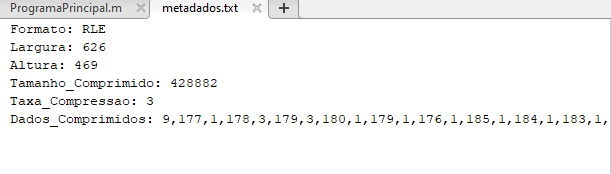
\includegraphics[width=\textwidth]{metadados.png}
        \caption{Parte dos metadados salvos no arquivo de texto}
        \label{fig:imagem3}
    \end{subfigure}
    \caption{Resultado visual dos experimentos}
    \label{fig:imagens}
\end{figure}

\section{Conclusão:}
Com base nas informações disponibilizadas acima, nota-se que um dos principais benefícios do RLE é sua simplicidade e eficácia na identificação e compactação de padrões repetidos, o que o torna uma escolha popular para aplicações onde a homogeneidade de cor é prevalente, como em logotipos, gráficos e imagens digitais com áreas de cores sólidas. Nessas situações, o RLE pode alcançar altas taxas de compressão, resultando em arquivos menores e economizando espaço de armazenamento ou largura de banda durante a transmissão.

No entanto, é importante observar que o desempenho do RLE pode ser prejudicado em imagens com variações complexas de cor ou padrões irregulares, onde a repetição de valores de cor não é tão evidente. Nessas circunstâncias, outras técnicas de compressão, como a compressão baseada em transformada (por exemplo, JPEG), podem ser mais adequadas para obter taxas de compressão mais eficientes.

Além disso, é crucial considerar o impacto do RLE na qualidade visual da imagem. Embora o RLE seja capaz de reduzir significativamente o tamanho do arquivo, a compressão excessiva pode levar a perdas perceptíveis na qualidade da imagem, especialmente em áreas de transição de cor ou detalhes finos.

Portanto, ao avaliar o impacto da homogeneidade de cor na eficiência do RLE, é importante realizar testes empíricos em uma variedade de imagens representativas do cenário de aplicação específico. Isso permitirá uma avaliação precisa do desempenho do RLE e sua adequação para a tarefa de compressão de imagens com características de homogeneidade de cor. 

\bibliographystyle{alpha}
\bibliography{sample}
\begin{enumerate}
    \item https://pt.wikipedia.org/wiki/Codifica%C3%A7%C3%A3o_run-length
    \item Salomon and Motta, Handbook of Data Compression, Springer
    \item https://www.cloudflare.com/pt-br/learning/performance/glossary/what-is-image-compression/
    \item https://nbviewer.org/github/leolca/notebooks
    \item https://www.wired.com/2009/03/racing-the-beam/
\end{enumerate}
\end{document}